% =============================================================
%  Writing New Molecules: A Transformer Autoencoder for SMILES
%  Series B: Deep Learning for Molecules, Post 6
%  Compiles with pdfLaTeX on Overleaf (no extra files needed).
% =============================================================
\documentclass[11pt]{article}

\usepackage[margin=1in]{geometry}
\usepackage[T1]{fontenc}
\usepackage{lmodern}
\usepackage{microtype}
\usepackage{amsmath,amssymb,bm}
\usepackage{booktabs}
\usepackage{enumitem}
\usepackage{xcolor}
\usepackage{listings}
\usepackage{tikz}
\usetikzlibrary{arrows.meta,positioning,calc}
\usepackage{pgfplots}
\pgfplotsset{compat=1.16}
\usepackage[most]{tcolorbox}
\usepackage[colorlinks=true,linkcolor=blue!50!black,urlcolor=blue!50!black]{hyperref}

\setlength{\parskip}{0.55em}
\setlength{\parindent}{0pt}

% ---------- macros ----------
\newcommand{\T}{\mathsf{T}}
\newcommand{\E}{\mathbb{E}}
\newcommand{\R}{\mathbb{R}}
\DeclareMathOperator{\softmax}{softmax}
\DeclareMathOperator{\Var}{Var}
\DeclareMathOperator{\MMD}{MMD}

% ---------- Colab links: edit these lines after you upload the notebooks to GitHub ----------
\newcommand{\colaburlfull}{https://colab.research.google.com/github/YOUR-USER/YOUR-REPO/blob/main/notebooks/VAE_Tutorial.ipynb}
\newcommand{\colaburlprimer}{https://colab.research.google.com/github/YOUR-USER/YOUR-REPO/blob/main/notebooks/B6_vae_primer_colab.ipynb}
\newcommand{\colabbutton}[2]{%
  \href{#1}{\tcbox[on line,colback=orange!15,colframe=orange!70!black,boxrule=0.6pt,arc=3pt,
    left=4pt,right=4pt,top=1pt,bottom=1pt]{\small\textbf{$\blacktriangleright$ #2}}}}
\newcommand{\tryit}[1]{\par\vspace{0.3em}\noindent
  \fcolorbox{orange!70!black}{orange!8}{\parbox{\dimexpr\linewidth-2\fboxsep-2\fboxrule\relax}{%
  \small $\blacktriangleright$ \textbf{Run it.} #1}}\par\vspace{0.3em}}

% ---------- code listings ----------
\definecolor{codebg}{RGB}{246,246,248}
\definecolor{codecomment}{RGB}{90,110,90}
\definecolor{codekw}{RGB}{30,60,160}
\lstset{
  language=Python,
  basicstyle=\ttfamily\small,
  keywordstyle=\color{codekw}\bfseries,
  commentstyle=\color{codecomment}\itshape,
  backgroundcolor=\color{codebg},
  frame=single,
  rulecolor=\color{black!15},
  breaklines=true,
  columns=fullflexible,
  showstringspaces=false,
  xleftmargin=0.5em,
  xrightmargin=0.5em,
  aboveskip=0.8em,
  belowskip=0.8em
}

% ---------- boxes ----------
\tcbuselibrary{skins,breakable}
\newtcolorbox{keybox}[1][]{
  enhanced, breakable, colback=blue!4, colframe=blue!50!black,
  fonttitle=\bfseries, title={#1}, boxrule=0.6pt, arc=2pt
}
\newtcolorbox{mathbox}[1][]{
  enhanced, breakable, colback=black!3, colframe=black!45,
  fonttitle=\bfseries, title={#1}, boxrule=0.6pt, arc=2pt
}
\newtcolorbox{warnbox}[1][]{
  enhanced, breakable, colback=red!4, colframe=red!60!black,
  fonttitle=\bfseries, title={#1}, boxrule=0.6pt, arc=2pt
}

% ---------- title ----------
\title{\textbf{Writing New Molecules:}\\[0.2em]
       A Transformer Autoencoder for SMILES}
\author{\textit{Series B: Deep Learning for Molecules --- Post 6 of 7}}
\date{}

\begin{document}
\maketitle
\thispagestyle{empty}

\begin{center}
\small
About 30 minutes of reading, plus the notebooks.\\
\textbf{Prerequisites:} Posts A1--A2 (gradient descent, neural networks); Post B5 (attention) helps but is not required.\\[0.5em]
\textbf{Notebook 1, the full tutorial:} \texttt{VAE\_Tutorial.ipynb} (GPU runtime, pre-trained model)\\
\textbf{Notebook 2, the primer:} \texttt{B6\_vae\_primer\_colab.ipynb} (CPU only, no model file)\\[0.4em]
\colabbutton{\colaburlfull}{Open the full tutorial}\quad
\colabbutton{\colaburlprimer}{Open the primer}\quad
{\footnotesize (see Section~\ref{sec:runit})}
\end{center}

\vspace{0.5em}
\hrule
\vspace{0.5em}

% =============================================================
\section{The question}
% =============================================================
The number of drug-like molecules is astronomically large, far too large to list or to screen one by one. A \textbf{generative model} tries a different route: learn what molecules ``look like'' from a large collection of examples, then \emph{sample} new ones.

The key observation of this post is that a molecule can be written as a line of text, a \textbf{SMILES string} such as \texttt{CC(=O)O} for acetic acid. Once molecules are text, we can borrow the machinery built for language, the \textbf{Transformer}. We will use one to compress each molecule into 1280 numbers (a \emph{latent vector}) and to rebuild it, and we will add one ingredient that turns this autoencoder into a generator: a rule that makes random numbers valid inputs.

Along the way we will test the model honestly. We measure not just how many generated strings are valid, but how they fail, how reliable the percentages are, and whether the latent space really does what the textbook says it should. One of those tests gives a surprise worth understanding.

\begin{keybox}[Where the numbers come from]
The model is the pre-trained Transformer autoencoder in the tutorial notebook of Prof.\ V.~S.~Batista's CHEM~584 course (an earlier version was designed by Dr.\ H.~Li). Data facts in Step~1 and all the mathematics are recomputed in the primer notebook. The chemistry numbers in Steps~6--9 (reconstruction, validity, and so on) are taken from the saved output of one run of the tutorial notebook on a T4 GPU with seed~0. Running it yourself will give numbers within the quoted error bars, not necessarily identical ones.
\end{keybox}

% =============================================================
\section{Step 1: Molecules as text}
% =============================================================
A \textbf{SMILES} string lists the atoms of a molecule and how they are bonded: atoms by their symbols, hydrogens left implicit, a double bond as \texttt{=}, a triple bond as \texttt{\#}, a branch in parentheses, a ring by a pair of matching digits, and an aromatic atom in lower case. The first molecule in our data set is
\begin{center}
\texttt{CC(C)(C)c1ccc2occ(CC(=O)Nc3ccccc3F)c2c1}
\end{center}
Our data are \textbf{249{,}455} drug-like molecules from the ZINC library, each with its SMILES string and three computed properties (logP, QED, SAS). The model learns from the strings alone.

A neural network reads numbers, not letters, so we convert each string to a row of integers:
\begin{enumerate}[nosep]
  \item \textbf{Markers.} Add a start character \texttt{!} and an end character \texttt{?}. The decoder starts from \texttt{!} and writes characters until it produces \texttt{?}. Without an end marker it would not know when to stop.
  \item \textbf{Dictionary.} Give every distinct character an integer, in order of first appearance. This data set has only \textbf{36} distinct characters (atoms, bonds, brackets, ring digits, and the two markers), so \texttt{!CC} becomes $[0,1,1]$.
  \item \textbf{Padding.} Pad every string to the longest one, \textbf{111} tokens, using a special padding token (index 36). The model \emph{masks} the padding so it is ignored.
\end{enumerate}

The padding is not a detail. The median string has only $46$ tokens, and $93.5\%$ of strings have $60$ or fewer; only $20$ of the 249{,}455 reach $100$ tokens. So about \textbf{58\%} of the padded matrix is padding. The data are split $90/10$: the first $224{,}509$ molecules train the model (cut into $876$ batches of $256$) and the last $24{,}946$ test it.

\tryit{Primer \S1. Reproduce every number above, including the token list of the first molecule, $[0,1,1,2,1,3,2,1,3,4,5,4,4,4,6,7,\dots]$.}

% =============================================================
\section{Step 2: A Transformer in one page}
% =============================================================
A SMILES string is a sentence in a strict language. A ring opened with the digit \texttt{1} must be closed by another \texttt{1}, parentheses must balance, and what is allowed for one atom depends on neighbors that may be far away in the string. The \textbf{Transformer} handles such long-range dependencies with \textbf{attention}.

The ingredients, in the order the code uses them:
\begin{itemize}[nosep]
  \item \textbf{Embeddings.} Each token and each \emph{position} becomes a learned vector of 128 numbers. Positions are needed because attention by itself does not know the order of the characters.
  \item \textbf{Self-attention.} Every position looks at all the others and takes a weighted average of their representations, with learned weights. With 4 \textbf{heads}, four such look-ups run in parallel, each on 32 of the 128 numbers.
  \item \textbf{Masks.} A \emph{padding mask} hides the padding tokens. In the decoder a \emph{causal mask} also hides all later positions, so that when predicting character $t$ the model can only use characters $1,\dots,t-1$.
  \item \textbf{Cross-attention.} Each decoder layer also attends to the encoder's output, here the 10 latent vectors of Step~3.
  \item \textbf{Residual connections, layer normalization and a small feed-forward network} around every sub-layer make a stack of 6 layers trainable.
\end{itemize}

The central formula, scaled dot-product attention, is derived in \hyperref[sec:S1]{Supplement S1}:
\begin{equation}
  \operatorname{Attention}(Q,K,V)=\softmax\!\Big(\frac{QK^{\T}}{\sqrt{d_k}}\Big)V,\qquad d_k=32 .
\end{equation}
The division by $\sqrt{d_k}$ is not cosmetic. Without it, the scores have variance $d_k$ and the softmax becomes nearly one-hot. In the primer, the average largest attention weight over $111$ keys is $0.675$ without the scaling and $0.075$ with it.

\tryit{Primer \S3. Check that $\Var(q\cdot k)=d_k$ and watch the softmax saturate without the scale.}

% =============================================================
\section{Step 3: Squeezing a molecule into 1280 numbers}
% =============================================================
Figure~\ref{fig:arch} shows the whole model. A string goes through the \textbf{encoder} (6 Transformer layers), which outputs one 128-number vector per position: $111\times128=14{,}208$ numbers. A single linear layer then squeezes these into the \textbf{latent vector} $\bm z$ of $10\times128=\textbf{1280}$ numbers. This bottleneck is the heart of the model. Everything the decoder knows about the molecule must pass through it.

\begin{figure}[ht]
\centering
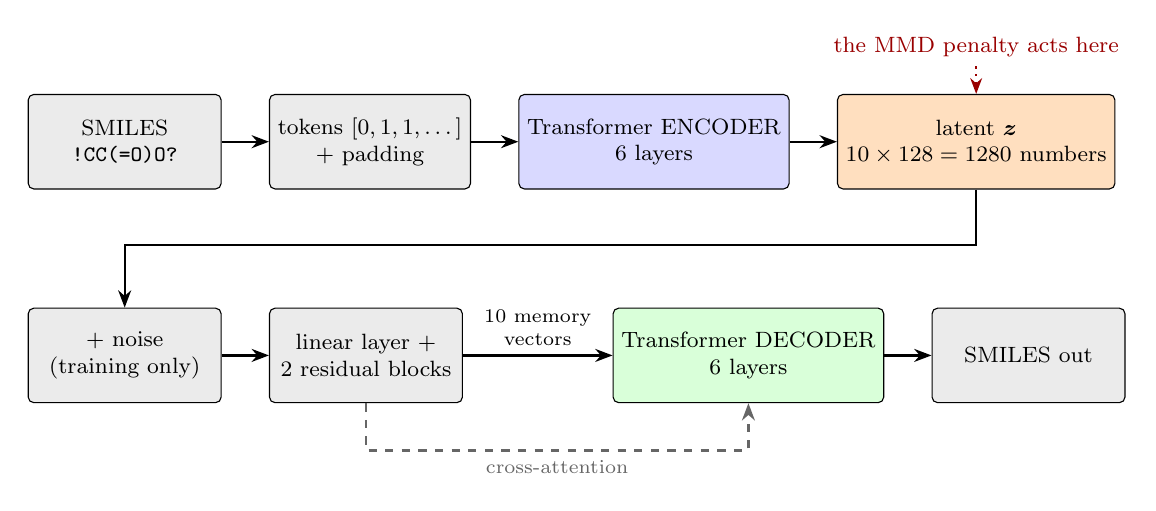
\begin{tikzpicture}[
  box/.style={draw, rounded corners=2pt, minimum height=1.2cm, minimum width=2.45cm, align=center, font=\footnotesize, inner sep=3pt},
  gray/.style={box, fill=black!8},
  enc/.style={box, fill=blue!15},
  dec/.style={box, fill=green!15},
  lat/.style={box, fill=orange!25},
  arr/.style={-{Stealth[length=2.2mm]}, thick}
]
% row 1: encoding
\node[gray] (smi) {SMILES\\\texttt{!CC(=O)O?}};
\node[gray, right=0.6cm of smi] (tok) {tokens $[0,1,1,\dots]$\\+ padding};
\node[enc, right=0.6cm of tok] (enc) {Transformer ENCODER\\6 layers};
\node[lat, right=0.6cm of enc] (z) {latent $\bm z$\\$10\times128=1280$ numbers};
\draw[arr] (smi) -- (tok); \draw[arr] (tok) -- (enc); \draw[arr] (enc) -- (z);
% row 2: decoding
\node[gray, below=1.5cm of smi] (noise) {$+$ noise\\(training only)};
\node[gray, right=0.6cm of noise] (inv) {linear layer $+$\\2 residual blocks};
\node[dec, right=1.9cm of inv] (dec) {Transformer DECODER\\6 layers};
\node[gray, right=0.6cm of dec] (out) {SMILES out};
\draw[arr] (z.south) -- ++(0,-0.7) -| (noise.north);
\draw[arr] (noise) -- (inv); \draw[arr] (inv) -- node[above, font=\scriptsize, align=center]{10 memory\\vectors} (dec); \draw[arr] (dec) -- (out);
\draw[arr, dashed, black!60] (inv.south) -- ++(0,-0.6) -| node[below, pos=0.25, font=\scriptsize] {cross-attention} (dec.south);
% MMD note
\node[font=\footnotesize, text=red!60!black, above=0.35cm of z] (mmd) {the MMD penalty acts here};
\draw[-{Stealth[length=2mm]}, red!60!black, dotted, thick] (mmd.south) -- (z.north);
\end{tikzpicture}
\caption{The model at a glance. The encoder compresses a string into a latent vector of 1280 numbers; the decoder rebuilds the string one character at a time, attending to ten 128-number ``memory'' vectors obtained from it. During training, Gaussian noise is added to $\bm z$ before decoding.}
\label{fig:arch}
\end{figure}

On the decoder side, $\bm z$ goes through a linear layer and is reshaped into 10 vectors of 128 numbers. Two small residual blocks mix these 10 vectors, and the decoder cross-attends to the result.

Counting parameters shows where the model's capacity sits (\hyperref[sec:S3]{Supplement S3} derives each line, and the total matches the $21{,}859{,}969$ printed by the tutorial):

\begin{center}
\small
\begin{tabular}{@{}lrr@{}}
\toprule
Component & Parameters & Share\\
\midrule
Embeddings (encoder and decoder) & $40{,}192$ & $0.2\%$\\
Encoder layers (6) & $794{,}880$ & $3.6\%$\\
Decoder layers (6) & $1{,}192{,}704$ & $5.5\%$\\
Decoder output layer & $4{,}773$ & $0.0\%$\\
\textbf{Latent layer} ($14{,}208\to1280$) & $18{,}187{,}520$ & $\mathbf{83.2\%}$\\
Inverse layer ($1280\to1280$) & $1{,}639{,}680$ & $7.5\%$\\
Two residual blocks & $220$ & $0.0\%$\\
\midrule
Total & $21{,}859{,}969$ & $100\%$\\
\bottomrule
\end{tabular}
\end{center}

Over four fifths of the parameters are in the one linear layer that forms the bottleneck. The Transformer layers themselves hold less than a tenth.

\tryit{Primer \S2. Derive the table from the architecture and confirm the total.}

% =============================================================
\section{Step 4: From an autoencoder to a generator}
% =============================================================
Trained on reconstruction alone, this model would be a plain \textbf{autoencoder}. It could rebuild training molecules very well, but its latent space would be irregular: the encoder is free to scatter molecules anywhere, so a \emph{random} vector usually lands in a region the decoder has never seen and decodes to nonsense. To generate, we need random vectors to be meaningful inputs.

A \textbf{variational autoencoder} fixes this by making the latent vectors of the whole data set look like draws from a simple \textbf{prior}, the standard normal $N(0,I)$ (mean $0$, variance $1$ in every direction). Then sampling $\bm z\sim N(0,I)$ and decoding gives new molecules.

The standard VAE enforces the prior with a KL-divergence term. This model uses a close relative, the \textbf{MMD autoencoder} (InfoVAE). The encoder outputs a single vector $\bm z$ per molecule, and a penalty on the \textbf{maximum mean discrepancy} between a batch of encoded vectors $\{\bm z_i\}$ and samples $\{\bm y_j\}$ from $N(0,I)$ pulls the \emph{collection} of latent vectors toward the prior. With a Gaussian kernel $k$,
\begin{equation}
  \MMD^2=\E\,k(\bm z,\bm z')+\E\,k(\bm y,\bm y')-2\,\E\,k(\bm z,\bm y).
  \label{eq:mmd}
\end{equation}
It is zero exactly when the two distributions agree (\hyperref[sec:S4]{Supplement S4}). The implementation in the tutorial keeps only the last, cross term:
\begin{equation}
  \text{penalty}=8\,\big[1-\overline{k(\bm z,\bm y)}\big],\qquad
  k(\bm x,\bm y)=\exp\!\Big(-\frac{\lVert\bm x-\bm y\rVert^2}{s}\Big),\quad s=d^2\cdot0.0005=819.2,
  \label{eq:simple}
\end{equation}
with $d=1280$. The tutorial flags this as a simplification and leaves the full estimator, Eq.~\eqref{eq:mmd}, as an exercise. Step~7 shows why the difference matters.

\textbf{Noise.} During training, Gaussian noise with standard deviation $1$ is added to $\bm z$ before decoding. The decoder then learns to cope with perturbed latent vectors, as it will when it decodes random draws. This also discourages \textbf{posterior collapse}, where the decoder ignores $\bm z$ and behaves as a plain language model.

The total loss is
\[
  \text{loss}=\underbrace{\text{cross-entropy}}_{\text{reconstruction, padding ignored}}+\underbrace{8\,[1-\overline{k(\bm z,\bm y)}]}_{\text{penalty toward the prior}} .
\]

% =============================================================
\section{Step 5: Training, briefly}
% =============================================================
During training the decoder receives the true string shifted by one position and must predict the next character at every position (\textbf{teacher forcing}); at generation time it feeds back its own predictions instead (\hyperref[sec:S2]{Supplement S2}). The optimizer is Adam with learning rate $5\times10^{-4}$, batch size $256$, and gradient clipping, and each training step compares the encoded batch with $1000$ fresh samples from $N(0,I)$.

Training from scratch takes about five minutes per epoch on a T4 GPU, and many epochs are needed. The method also needs care: with a \emph{small} penalty weight the model reconstructs well but random vectors decode poorly, and with a \emph{large} weight sampling works but reconstructions suffer. In practice one starts small and increases the weight while watching both. For this reason the tutorial ships a pre-trained model and does not recommend retraining. (The notebook's training cell uses a fixed weight; how the shipped model's weight was scheduled is not documented there.)

% =============================================================
\section{Step 6: Reconstruction}
% =============================================================
First test: encode a molecule, decode its latent vector, compare. The first molecule of the data set is reconstructed exactly, character for character. Across $5000$ test molecules, however, only $3429$ come back identical, a reconstruction accuracy of $\mathbf{68.6\%}$ ($\pm1.3$ points at 95\% confidence).

That is worth pausing on: about a third of test molecules come back \emph{changed}. A SMILES string that differs in one position describes a different molecule, possibly with different properties. We will see an example in Step~9.

% =============================================================
\section{Step 7: Does the latent space match its prior?}
% =============================================================
The penalty is supposed to make the latent vectors of real molecules look like draws from $N(0,I)$. How do we check? A tempting test is the histogram of the first principal component, but it misleads for small samples. With $n$ points in $d$ dimensions, perfect $N(0,I)$ data has a first principal component with standard deviation about $1+\sqrt{d/n}$, not $1$ (Supplement~\hyperref[sec:S6]{S6}). For $n=256$, $d=1280$ that is $3.2$. The fair test compares the encoded vectors with a \textbf{null reference}: random $N(0,I)$ draws of the same size, analyzed the same way.

The tutorial's diagnostics, for 2000 encoded test molecules, give a clear answer:

\begin{center}
\begin{tabular}{@{}lcc@{}}
\toprule
 & Encoded molecules & Prior $N(0,I)$\\
\midrule
Mean vector length $\lVert\bm z\rVert$ & $14.3$ & $35.8$\\
Mean standard deviation of a coordinate & $0.39$ & $1$\\
Penalty value (Eq.~\ref{eq:simple}) vs.\ the prior & $6.672$ & $7.641$ (prior vs.\ prior)\\
\bottomrule
\end{tabular}
\end{center}

\textbf{The encoded vectors do not match the prior.} They are much shorter and much less spread out. Yet the model generates valid molecules from random draws about $79\%$ of the time (Step~8). How can both be true?

\subsection*{What the simplified penalty actually enforces}
The cross term alone rewards latent vectors that are close to the prior samples \emph{on average}. If the vectors $\bm z$ have spread $\sigma$ in every coordinate, the penalty has a closed form (\hyperref[sec:S4]{Supplement S4}):
\begin{equation}
  \text{penalty}(\sigma)=8\Big[1-\Big(1+\tfrac{2(\sigma^2+1)}{s}\Big)^{-d/2}\Big],
\end{equation}
which \emph{increases} with $\sigma$. The lowest penalty is at $\sigma=0$: all vectors collapsed onto the origin. The full $\MMD^2$ of Eq.~\eqref{eq:mmd}, in contrast, has its minimum exactly at $\sigma=1$. Figure~\ref{fig:pen} plots both.

\begin{figure}[ht]
\centering
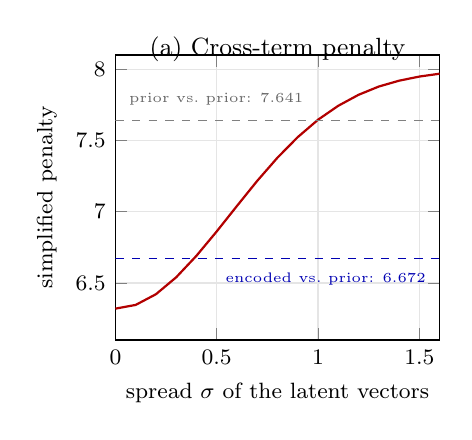
\begin{tikzpicture}
\begin{axis}[width=0.47\textwidth, height=5.2cm, xlabel={spread $\sigma$ of the latent vectors}, ylabel={simplified penalty},
  title={\small (a) Cross-term penalty}, ymin=6.1, ymax=8.1, xmin=0, xmax=1.6, grid=major, grid style={black!10},
  every axis title/.style={at={(0.5,1.02)}}, tick label style={font=\footnotesize}, label style={font=\footnotesize}]
\addplot[red!70!black, thick] coordinates {(0.0,6.320) (0.1,6.346) (0.2,6.421) (0.3,6.540) (0.4,6.691) (0.5,6.862) (0.6,7.041) (0.7,7.217) (0.8,7.380) (0.9,7.524) (1.0,7.646) (1.1,7.744) (1.2,7.821) (1.3,7.879) (1.4,7.920) (1.5,7.949) (1.6,7.969)};
\addplot[black!50, dashed] coordinates {(0,7.641) (1.6,7.641)};
\addplot[blue!70!black, dashed] coordinates {(0,6.672) (1.6,6.672)};
\node[font=\tiny, anchor=south west, black!60] at (axis cs:0.02,7.68) {prior vs.\ prior: 7.641};
\node[font=\tiny, anchor=north east, blue!70!black] at (axis cs:1.58,6.64) {encoded vs.\ prior: 6.672};
\end{axis}
\end{tikzpicture}\hfill
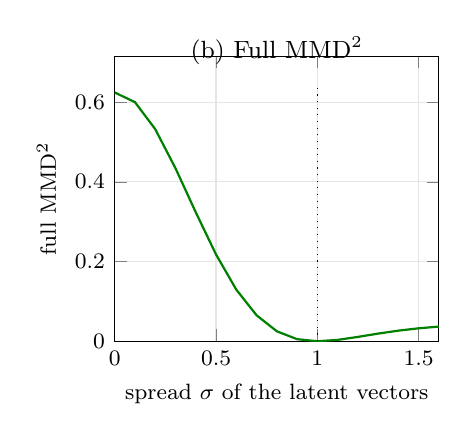
\begin{tikzpicture}
\begin{axis}[width=0.47\textwidth, height=5.2cm, xlabel={spread $\sigma$ of the latent vectors}, ylabel={full $\MMD^2$},
  title={\small (b) Full MMD$^2$}, ymin=0, xmin=0, xmax=1.6, grid=major, grid style={black!10},
  every axis title/.style={at={(0.5,1.02)}}, tick label style={font=\footnotesize}, label style={font=\footnotesize}]
\addplot[green!50!black, thick] coordinates {(0.0,0.6243) (0.1,0.6000) (0.2,0.5321) (0.3,0.4341) (0.4,0.3236) (0.5,0.2178) (0.6,0.1295) (0.7,0.0652) (0.8,0.0250) (0.9,0.0052) (1.0,0.0000) (1.1,0.0034) (1.2,0.0109) (1.3,0.0192) (1.4,0.0266) (1.5,0.0325) (1.6,0.0368)};
\addplot[black, dotted] coordinates {(1,0) (1,0.65)};
\end{axis}
\end{tikzpicture}
\caption{(a) The model's simplified penalty, for latent vectors with spread $\sigma$ in every coordinate, falls as the vectors shrink toward the origin. The two dashed lines are the values measured on the tutorial's encoded molecules (blue) and on two prior samples (grey). (b) The full $\MMD^2$ vanishes only at $\sigma=1$, when the distributions match. Curves are the closed forms of Supplement~S4.}
\label{fig:pen}
\end{figure}

The numbers agree strikingly. Solving the closed form for the measured penalty of $6.672$ gives $\sigma=0.388$, against a measured mean coordinate spread of $0.39$. The prior-vs-prior reference comes out at $7.646$ against $7.641$ measured. (Real latent coordinates are not all equally spread, so treat this as a confirmation of the mechanism and not as an exact identity.) This is a good example of a general lesson: \textbf{a loss named ``MMD'' is not the MMD unless all its terms are there}, and measuring the diagnostics is how you find out.

\subsection*{Why random sampling still works}
The answer lies in the noise of Step~4. During training the decoder never sees $\bm z$ itself, but $\bm z+\bm\varepsilon$ with $\bm\varepsilon\sim N(0,I)$. If the encoder's coordinates have spread $0.39$, the decoder's training input has per-coordinate spread $\sqrt{0.39^2+1}=1.07$, so its length is about $\sqrt{1280\cdot1.152}=38.4$. A draw from the prior has length $\sqrt{1280}=35.8$. The two are within 7\%. The noise makes the decoder's training inputs look almost like prior samples, even though the encoder's own outputs do not.

\begin{center}
\small
\begin{tabular}{@{}lc@{}}
\toprule
Vector & Typical length\\
\midrule
Encoder output $\bm z$ (measured $14.3$) & $\approx14$\\
Decoder training input $\bm z+\bm\varepsilon$ & $\approx38.4$\\
Decoder sampling input, a draw from $N(0,I)$ & $\approx35.8$\\
\bottomrule
\end{tabular}
\end{center}

This explanation fits the numbers, but it is a hypothesis; we have not tested it on the model. It makes a testable prediction (Exercise~5): validity should peak when you sample $\bm z\sim N(0,\sigma^2I)$ with $\sigma$ near $1.07$ and fall off on both sides.

\tryit{Primer \S4--6. Reproduce Figure~\ref{fig:pen} from the closed forms, confirm them by Monte Carlo (agreement to three digits), and compute the three lengths above.}

% =============================================================
\section{Step 8: Sampling new molecules, and judging them honestly}
% =============================================================
Now the real test. Draw $5000$ random vectors from $N(0,I)$, decode them, and measure. We follow the standard metrics of the field (the MOSES and GuacaMol benchmarks):

\begin{center}
\small
\begin{tabular}{@{}lccc@{}}
\toprule
Metric & Count & Out of & Percent (95\% CI)\\
\midrule
Parses as SMILES (grammar only) & $4347$ & $5000$ & $86.94\pm0.93$\\
\textbf{Chemically valid} & $3971$ & $5000$ & $\mathbf{79.42}\pm1.12$\\
Repeated (among valid) & $161$ & $3971$ & $4.05\pm0.61$\\
Novel (among distinct valid) & $3803$ & $3810$ & $99.82\pm0.14$\\
Exactly reconstructed (test) & $3429$ & $5000$ & $68.58\pm1.29$\\
\bottomrule
\end{tabular}
\end{center}

``Parses'' means RDKit can read the string; ``chemically valid'' also requires that it pass RDKit's sanitization (valence rules, aromaticity), which is the validity that matters. ``Novel'' means the canonical SMILES is not among the 250{,}000 training molecules. Canonicalizing first matters: the same molecule written in a different atom order is still the same molecule.

Three ways to read this table well:
\begin{enumerate}[nosep]
  \item \textbf{Combine the rows.} Validity $\times$ uniqueness $\times$ novelty is the yield of \emph{new, distinct, valid} molecules: $0.7942\times0.9595\times0.9982=76.06\%$, that is $3803$ of the $5000$ draws.
  \item \textbf{Respect the error bars.} They come from a finite sample, $1.96\sqrt{p(1-p)/n}$. These are single draws with a fixed seed; another seed gives numbers within the margins.
  \item \textbf{Do not over-read ``novel.''} ZINC is a tiny part of chemical space, so almost any reasonable molecule is ``not in ZINC.'' Novelty does not mean new to chemistry, nor interesting.
\end{enumerate}

\subsection*{How do the failures fail?}
Of the $5000$ strings, $79.42\%$ are valid. The rest fail in three different ways:

\begin{center}
\small
\begin{tabular}{@{}lrl@{}}
\toprule
Outcome & Percent & Meaning\\
\midrule
Syntax error & $13.06$ & unbalanced brackets or unclosed rings, not a legal SMILES\\
Kekulization error & $7.24$ & an aromatic ring cannot be written with alternating bonds\\
Valence error & $0.28$ & an atom has too many bonds\\
\bottomrule
\end{tabular}
\end{center}

(The Kekulization row combines two exception types of $7.20\%$ and $0.04\%$.) The dominant failures are \emph{grammatical}: a character-by-character generator opens a ring or a bracket and does not always close it. This is exactly the long-range bookkeeping of Step~2, and it is why alternative string representations designed to be always valid, such as SELFIES, exist (Supplement~\hyperref[sec:S9]{S9}).

\subsection*{Do the generated molecules resemble the training data?}
Validity and novelty say nothing about whether new molecules are \emph{like} the training ones, which was the goal. Comparing property distributions (computed with RDKit for both sets) for the novel generated molecules and $5000$ random ZINC molecules:

\begin{center}
\begin{tabular}{@{}lcc@{}}
\toprule
 & ZINC (5000) & Generated (novel, valid)\\
\midrule
logP, mean $\pm$ std & $2.47\pm1.42$ & $2.65\pm1.27$\\
QED, mean $\pm$ std & $0.73\pm0.14$ & $0.81\pm0.10$\\
\bottomrule
\end{tabular}
\end{center}

The generated molecules have a higher average QED (``drug-likeness'') and a \emph{narrower} spread in both properties. The generator is biased toward the typical, and may be less diverse than its training data. A common reason is that sampling favors high-probability, average-looking structures, though we have not tested that here.

\begin{warnbox}[A valid molecule is not a good molecule]
Passing RDKit's valence checks does not make a structure stable, synthesizable or useful, and ``not in this 250k set'' does not mean ``never seen.'' Any real application needs further filtering (synthetic-accessibility and property scores, substructure alerts) and expert review.
\end{warnbox}

% =============================================================
\section{Step 9: Walking from ibuprofen to caffeine}
% =============================================================
Because the latent space is continuous, we can walk from the latent vector of one molecule to that of another and decode the points on the way. The tutorial uses \textbf{ibuprofen} and \textbf{caffeine}, with 7 equally spaced points $\bm z_I+\tfrac{i}{6}(\bm z_C-\bm z_I)$, $i=0,\dots,6$.

First, the end points. Caffeine is reconstructed exactly. Ibuprofen is not: the decoded molecule is \texttt{CC(C)CC1=CC=CC(=C1)C(C)C(=O)O}, which has the isobutyl and propionic-acid groups on the \emph{meta} rather than the \emph{para} positions of the benzene ring, a structural isomer. Here is Step~6's imperfect reconstruction made concrete. The walk uses the latent vectors of the \emph{true} ibuprofen and caffeine.

In the tutorial's run, the path (Tanimoto similarity to both end points is plotted in the notebook) goes: step~0, the meta isomer of ibuprofen; step~1, true ibuprofen; steps~2 and 3, molecules that are neither; step~4, an invalid string; step~5, a close analogue of caffeine; step~6, caffeine. The molecules change gradually from one end to the other, though a few intermediates are chemically odd. Different models, or paths in other directions, give different intermediates.

A geometric caution (\hyperref[sec:S8]{Supplement S8}): in $1280$ dimensions, a straight line between two prior-like vectors passes through points that are shorter than any typical draw. Its midpoint has length $\approx25.3$ instead of $35.8$, a factor of $1/\sqrt2$. Spherical interpolation (\emph{slerp}) avoids this. Whether it helps for this model is Exercise~6.

\tryit{Full tutorial \S7. Run the walk and the similarity plot. Primer \S8. Watch the length of the interpolated vector shrink to $25.3$ for straight-line interpolation and stay at $35.8$ for slerp.}

% =============================================================
\section{Run it yourself in Colab}
\label{sec:runit}
% =============================================================
Two notebooks accompany this post, for different purposes.

\begin{keybox}[Which notebook?]
\begin{description}[leftmargin=0pt, nosep, labelindent=0pt]
  \item[Primer] \colabbutton{\colaburlprimer}{Open the primer}\ \ \texttt{B6\_vae\_primer\_colab.ipynb}. CPU only, about a minute, no model file. It reproduces every data fact, the parameter count, and all of the mathematics of Steps~2--9, and ends with a self-check cell. Start here.
  \item[Full tutorial] \colabbutton{\colaburlfull}{Open the full tutorial}\ \ \texttt{VAE\_Tutorial.ipynb}. Needs a \textbf{GPU runtime} (a T4 is enough) and the pre-trained model file. It runs the model: reconstruction, sampling, the validity tables, 3D molecule views, and the ibuprofen--caffeine walk.
\end{description}
\end{keybox}

\begin{warnbox}[Security note on the model file]
The pre-trained model is distributed as \texttt{VAE\_transformer\_model.pckl}, a Python \emph{pickle}. A pickle can execute arbitrary code when loaded, so load one only if you received it from a source you trust. The full tutorial also accepts a weights-only file, \texttt{VAE\_transformer\_state\_dict.pt}, loaded with \texttt{weights\_only=True}, which contains only numbers. It has a cell that exports one from a trusted pickle. Prefer that format for sharing.
\end{warnbox}

\subsection{Where each step lives}
\begin{center}
\small
\begin{tabular}{@{}llp{6.4cm}@{}}
\toprule
Post & Notebook & What you should see\\
\midrule
Step 1 & Primer \S1 & $249{,}455$ molecules, $36$ characters, $58.3\%$ padding, $876$ batches\\
Step 2 & Primer \S3 & $\Var(q\cdot k)\approx32$; largest attention weight $0.675\to0.075$\\
Step 3 & Primer \S2 & Parameter table totaling $21{,}859{,}969$; latent layer $83.2\%$\\
Step 4--5 & Full \S4--5 & Model definition, loading, optional training\\
Step 6 & Full \S6.1 & First molecule reconstructed exactly\\
Step 7 & Primer \S4--6 & Penalty vs.\ $\sigma$; lengths $14.0$, $38.4$, $35.8$. Full \S6.2 for the real latent space\\
Step 8 & Primer \S7; Full \S6.3 & The metrics table with error bars; failure types; properties\\
Step 9 & Primer \S8; Full \S7 & Interpolation geometry; the ibuprofen--caffeine walk\\
\bottomrule
\end{tabular}
\end{center}

\subsection{The key calculation in one cell}
The heart of Step~7 needs no data and no model. This script uses only NumPy:

\begin{lstlisting}
import numpy as np

d = 1280
s = d * d * 0.0005                                   # kernel: k(x, y) = exp(-|x - y|^2 / s)
cross  = lambda sx: (1 + 2 * (sx**2 + 1) / s) ** (-d / 2)     # E k(z, y) for z ~ N(0, sx^2 I), y ~ N(0, I)
simple = lambda sx: 8 * (1 - cross(sx))                       # the model's simplified penalty
full   = lambda sx: (1 + 4 * sx**2 / s) ** (-d / 2) + (1 + 4 / s) ** (-d / 2) - 2 * cross(sx)   # full MMD^2

for sx in (0.0, 0.39, 0.7, 1.0, 1.5):
    print(f"sigma = {sx:4.2f}: simplified penalty = {simple(sx):6.3f}   full MMD^2 = {full(sx):+.5f}")
print("measured in the full tutorial: encoded vs prior 6.672, prior vs prior 7.641")

sz = 0.39                                             # measured spread of the encoder output
print("\nlengths: encoder output %.1f | decoder training input %.1f | prior draw %.1f"
      % (d**0.5 * sz, (d * (sz**2 + 1)) ** 0.5, d**0.5))
\end{lstlisting}

Expected output:
\begin{lstlisting}[language={},basicstyle=\ttfamily\small]
sigma = 0.00: simplified penalty =  6.320   full MMD^2 = +0.62425
sigma = 0.39: simplified penalty =  6.674   full MMD^2 = +0.33469
sigma = 0.70: simplified penalty =  7.217   full MMD^2 = +0.06515
sigma = 1.00: simplified penalty =  7.646   full MMD^2 = +0.00000
sigma = 1.50: simplified penalty =  7.949   full MMD^2 = +0.03248
measured in the full tutorial: encoded vs prior 6.672, prior vs prior 7.641

lengths: encoder output 14.0 | decoder training input 38.4 | prior draw 35.8
\end{lstlisting}

Note how the second column falls toward $\sigma=0$ while the third column is smallest at $\sigma=1$: that is Figure~\ref{fig:pen} in six lines.

% =============================================================
\section{What to take away}
% =============================================================
\begin{keybox}[Summary]
\begin{itemize}[nosep]
  \item A molecule written as a SMILES string can be modeled with the machinery built for language: tokens, embeddings, attention, a Transformer encoder and decoder.
  \item A plain autoencoder reconstructs but cannot generate. A \textbf{prior} on the latent space, enforced by a penalty such as MMD, makes random vectors meaningful.
  \item Check the latent space against a \textbf{null reference}, not against intuition. Here the encoded vectors are far shorter than the prior (14 vs.\ 36), because the \emph{cross-term-only} penalty pulls vectors toward the origin.
  \item Noise added during training explains why sampling still works: the decoder's training inputs look almost like prior samples.
  \item Evaluate a generator with validity, uniqueness, novelty, \textbf{error bars}, a look at \emph{how} it fails, and property distributions, not a single percentage.
  \item Reconstruction is imperfect (68.6\% exact), a valid molecule is not necessarily a good one, and straight-line interpolation in high dimension leaves the typical region.
\end{itemize}
\end{keybox}

\textbf{Next in the series (B7):} predicting dynamics with dynamic mode decomposition.

\vspace{0.5em}
{\footnotesize\textbf{Credits and license.} The tutorial notebook, \textit{VAE Transformer: De novo generation of molecules}, is by Prof.\ Victor S.\ Batista (CHEM~584, Yale), version~1.0, November 2026; an earlier version of the assignment was designed by Dr.\ Haote Li. Text is CC~BY~4.0 and code is MIT, per the notebook. The ZINC subset is distributed with the \texttt{chemical\_vae} repository of the Aspuru-Guzik group.}

\clearpage
% =============================================================
\section*{Supplementary Reading: The Math}
\addcontentsline{toc}{section}{Supplementary Reading: The Math}
% =============================================================
\textit{Prerequisites: matrix products, expectations and variances of Gaussians, and the chain rule (Toolbox T1--T3). Post A2 for backpropagation.}

\phantomsection\label{sec:S1}
\subsection*{S1. Scaled dot-product attention}
Let the query, key and value matrices be $Q\in\R^{n_q\times d_k}$, $K\in\R^{n_k\times d_k}$, $V\in\R^{n_k\times d_v}$. Each row of the \textbf{score matrix} $S=QK^{\T}/\sqrt{d_k}$ is turned into weights by a softmax, and the output is the weighted average of the rows of $V$:
\[
  A=\softmax(S)\ \text{(row-wise)},\qquad \operatorname{Attention}(Q,K,V)=AV,\qquad A_{ij}=\frac{e^{S_{ij}}}{\sum_{j'}e^{S_{ij'}}} .
\]

\paragraph{Why $\sqrt{d_k}$.} Suppose a query $\bm q$ and a key $\bm k$ have independent entries of mean $0$ and variance $1$. Then
\[
  \E[\bm q\cdot\bm k]=0,\qquad
  \Var(\bm q\cdot\bm k)=\sum_{i=1}^{d_k}\Var(q_ik_i)=d_k ,
\]
since $\Var(q_ik_i)=\E[q_i^2]\E[k_i^2]=1$. Dividing by $\sqrt{d_k}$ restores unit variance. Without it the scores have standard deviation $\sqrt{32}\approx5.7$, the softmax is nearly one-hot, and its gradients are close to zero, which makes learning slow (the same issue as saturating activations in Post A3).

\paragraph{Masks.} A mask is applied by adding $-\infty$ (in the code, $-10^{10}$) to the forbidden entries of $S$ before the softmax, which sends their weights to $0$. The causal mask forbids $j>i$, so the weights of position $i$ depend only on positions $\le i$.

\paragraph{Multi-head attention.} With $h=4$ heads, the $128$-dimensional vectors are projected, split into $4$ blocks of $d_k=32$, attention is applied to each block, and the results are concatenated and projected again:
\[
  \operatorname{MHA}(X)=\big[\operatorname{head}_1;\dots;\operatorname{head}_4\big]W_O,\qquad
  \operatorname{head}_a=\operatorname{Attention}(XW_Q^{(a)},XW_K^{(a)},XW_V^{(a)}) .
\]
The four projections $W_Q,W_K,W_V,W_O$ are $128\times128$ matrices with biases, $4\,(128^2+128)=66{,}048$ parameters per attention block.

\phantomsection\label{sec:S2}
\subsection*{S2. Autoregressive decoding and teacher forcing}
A string $\bm s=(s_1,\dots,s_T)$ (with markers) is modeled by the chain rule of probability,
\[
  p(\bm s\mid\bm z)=\prod_{t=1}^{T}p(s_t\mid s_{<t},\bm z).
\]
The decoder outputs, at each position, a probability vector over the 37 tokens (a softmax of its final linear layer). Training minimizes the average cross-entropy, ignoring padding,
\[
  \mathcal L_{\rm CE}=-\frac1{|\mathcal T|}\sum_{(\text{molecule},t)\in\mathcal T}\ln p(s_t\mid s_{<t},\bm z),
\]
where $\mathcal T$ is the set of non-padding positions. In \textbf{teacher forcing} the conditioning prefix $s_{<t}$ is the \emph{true} prefix, so all $T$ terms are computed in one parallel pass using the causal mask (the code feeds \texttt{trg[:, :-1]} and compares with \texttt{trg[:, 1:]}). At generation time the true prefix is unavailable, so the model feeds back its own choices. The tutorial uses \textbf{greedy decoding}, $s_t=\arg\max p(\cdot\mid s_{<t},\bm z)$. Sampling from the predicted distribution (with a temperature) instead gives a different validity--diversity trade-off.

\phantomsection\label{sec:S3}
\subsection*{S3. Counting the parameters}
A linear layer from $m$ to $n$ units has $mn+n$ parameters; a layer normalization over $n$ units has $2n$; an embedding table with $r$ rows of width $H$ has $rH$. With $H=128$, feed-forward width $256$, $37$ tokens, $120$ positions:
\begin{align*}
  \text{embeddings (each of enc., dec.)} &= 37\cdot128+120\cdot128=20{,}096,\\
  \text{attention block} &= 4(128^2+128)=66{,}048,\\
  \text{feed-forward block} &= (128\cdot256+256)+(256\cdot128+128)=65{,}920,\\
  \text{encoder layer} &= 2\cdot256+66{,}048+65{,}920=132{,}480,\\
  \text{decoder layer} &= 3\cdot256+2\cdot66{,}048+65{,}920=198{,}784 .
\end{align*}
(The decoder layer has two attention blocks, self- and cross-attention, and three layer norms.) Adding the six-layer stacks and the remaining pieces,
\begin{align*}
  \text{encoder}&=20{,}096+6\cdot132{,}480=814{,}976,\\
  \text{decoder}&=20{,}096+6\cdot198{,}784+(128\cdot37+37)=1{,}217{,}573,\\
  \text{latent layer}&=14{,}208\cdot1280+1280=18{,}187{,}520,\\
  \text{inverse layer}&=1280^2+1280=1{,}639{,}680,\\
  \text{residual blocks}&=2\,(10^2+10)=220,\\
  \text{total}&=814{,}976+1{,}217{,}573+18{,}187{,}520+1{,}639{,}680+220=21{,}859{,}969 .
\end{align*}
Note that the latent layer's input size is $111\cdot128=14{,}208$ (padded length times embedding width), not $120\cdot128$: the position table has room for $120$ positions but the data fill $111$. The latent layer holds $18{,}187{,}520/21{,}859{,}969=83.2\%$ of all parameters.

\phantomsection\label{sec:S4}
\subsection*{S4. MMD, and what the simplified penalty enforces}
\paragraph{Definition.} For distributions $P,Q$ and a kernel $k$, the \textbf{maximum mean discrepancy} is the distance between the mean embeddings of $P$ and $Q$ in the kernel's feature space:
\[
  \MMD^2(P,Q)=\E_{\bm z,\bm z'\sim P}\,k(\bm z,\bm z')+\E_{\bm y,\bm y'\sim Q}\,k(\bm y,\bm y')-2\,\E_{\bm z\sim P,\ \bm y\sim Q}\,k(\bm z,\bm y).
\]
For a \emph{characteristic} kernel such as the Gaussian, $\MMD^2(P,Q)=0$ if and only if $P=Q$ (Gretton et al., 2012). Given samples $\{\bm z_i\}_{i\le n}$ and $\{\bm y_j\}_{j\le m}$, the unbiased estimate replaces each expectation by an average, leaving out the diagonal terms $i=i'$ in the two same-sample sums.

\paragraph{Closed form for Gaussians.} Let $k(\bm x,\bm y)=\exp(-\lVert\bm x-\bm y\rVert^2/s)$, $\bm z\sim N(0,\sigma_z^2I_d)$ and $\bm y\sim N(0,\sigma_y^2I_d)$ independent. Then $\bm z-\bm y\sim N(0,(\sigma_z^2+\sigma_y^2)I_d)$, so $\lVert\bm z-\bm y\rVert^2=(\sigma_z^2+\sigma_y^2)\,X$ with $X\sim\chi^2_d$. The moment generating function of $\chi^2_d$ is $\E[e^{-tX}]=(1+2t)^{-d/2}$, so with $t=(\sigma_z^2+\sigma_y^2)/s$:
\begin{equation}
  \E\,k(\bm z,\bm y)=\Big(1+\frac{2(\sigma_z^2+\sigma_y^2)}{s}\Big)^{-d/2}.
\end{equation}
The same formula with both variances equal to $\sigma_z^2$, respectively $\sigma_y^2$, gives the other two terms:
\[
  \MMD^2=\Big(1+\tfrac{4\sigma_z^2}{s}\Big)^{-d/2}+\Big(1+\tfrac{4\sigma_y^2}{s}\Big)^{-d/2}-2\Big(1+\tfrac{2(\sigma_z^2+\sigma_y^2)}{s}\Big)^{-d/2}.
\]
Putting $\sigma_z=\sigma_y$ makes all three terms equal and $\MMD^2=0$, as it must.

\paragraph{The model's kernel.} The code computes $\exp(-\tfrac{1}{d\cdot0.0005}\cdot\tfrac1d\lVert\bm x-\bm y\rVert^2)$, which is the kernel above with $s=d^2\cdot0.0005=1280^2\cdot0.0005=819.2$.

\paragraph{Direction of the pull.} Take $\sigma_y=1$ and write $g(\sigma)=\big(1+2(\sigma^2+1)/s\big)^{-d/2}$. Since the base is increasing in $\sigma$ and the exponent $-d/2$ is negative, $g$ is strictly \emph{decreasing} in $\sigma$, so the simplified penalty $8(1-g(\sigma))$ is strictly \emph{increasing}: its minimum is at $\sigma=0$. In numbers: $6.320$ at $\sigma=0$, $6.674$ at $\sigma=0.39$, $7.646$ at $\sigma=1$. The penalty keeps pulling the vectors toward the origin, whereas the full $\MMD^2$ is minimized at $\sigma=1$. The cross-entropy loss pushes back, because the decoder needs the latent vectors to carry information, and the encoder settles at a compromise. We showed the \emph{direction} of the pull and that a spread of $0.39$ reproduces the measured value; where the equilibrium lies is empirical.

\phantomsection\label{sec:S5}
\subsection*{S5. Lengths of Gaussian vectors, and the noise argument}
For $\bm y\sim N(0,I_d)$, $\lVert\bm y\rVert^2\sim\chi^2_d$ has mean $d$ and variance $2d$. By the delta method, $\lVert\bm y\rVert$ has mean $\approx\sqrt d$ and standard deviation $\approx\sqrt{2d}/(2\sqrt d)=1/\sqrt2\approx0.71$. For $d=1280$: $35.8\pm0.7$, which matches simulation ($35.76\pm0.71$). A draw from the prior sits on a thin shell, not near the origin.

If $\bm z$ has independent coordinates of variance $\sigma_z^2$ and noise $\bm\varepsilon\sim N(0,I)$ is added, each coordinate of $\bm z+\bm\varepsilon$ has variance $\sigma_z^2+1$ and the length is concentrated near $\sqrt{d(\sigma_z^2+1)}$. For $\sigma_z=0.39$: $\sqrt{1280\cdot1.152}=38.4$. The ratio to the prior's shell is $\sqrt{1.152}=1.073$. This is the sense in which the noise makes the decoder's training inputs ``look like'' prior samples. It is an argument about typical lengths, not a proof that the decoder generalizes to every point of the shell; Exercise~5 tests it.

\phantomsection\label{sec:S6}
\subsection*{S6. The null reference for principal components}
For $n$ samples of $N(0,I_d)$, the sample covariance has eigenvalues spread over the Marchenko--Pastur interval; its largest eigenvalue converges, for $d/n\to c$, to $(1+\sqrt c)^2$. The standard deviation along the first principal component is therefore about $1+\sqrt{d/n}$. For $d=1280$:
\begin{center}
\small
\begin{tabular}{@{}rcc@{}}
\toprule
$n$ & Predicted $1+\sqrt{d/n}$ & Simulated\\
\midrule
256 & $3.24$ & $3.20$\\
2000 & $1.80$ & $1.80$\\
\bottomrule
\end{tabular}
\end{center}
So a wide first-PC histogram from a few hundred molecules says nothing by itself. Compare with the same analysis of random $N(0,I)$ data of the same size.

\phantomsection\label{sec:S7}
\subsection*{S7. Evaluation metrics and their error bars}
Let $n$ strings be sampled, $n_v$ of them valid, $n_d$ distinct among the valid, and $n_n$ of those novel. Then
\[
  \text{validity}=\frac{n_v}{n},\quad
  \text{uniqueness}=\frac{n_d}{n_v},\quad
  \text{novelty}=\frac{n_n}{n_d},\quad
  \text{yield}=\frac{n_n}{n}=\text{validity}\times\text{uniqueness}\times\text{novelty}.
\]
For $n=5000$: $n_v=3971$, $n_d=3810$, $n_n=3803$, giving $0.7942\times0.9595\times0.9982=0.7606$.

\paragraph{Normal-approximation interval.} A count $k$ out of $n$ has proportion $\hat p=k/n$ with standard error $\sqrt{\hat p(1-\hat p)/n}$, so the approximate 95\% interval is $\hat p\pm1.96\sqrt{\hat p(1-\hat p)/n}$. For validity, $1.96\sqrt{0.7942\cdot0.2058/5000}=0.0112$, that is $\pm1.12$ points. The width shrinks as $1/\sqrt n$: halving it takes four times as many samples. The approximation is poor near $0$ or $1$ with few samples, where a Wilson interval is better.

\paragraph{A caveat about uniqueness.} Uniqueness is not a fixed property of the model. As the number of samples grows, repeats become more likely (a birthday-problem effect), so uniqueness measured on $5000$ draws overstates what you would see with $10^6$.

\phantomsection\label{sec:S8}
\subsection*{S8. Interpolation in high dimension}
Let $\bm a,\bm b$ be independent $N(0,I_d)$ vectors and consider the straight line $\bm z(t)=(1-t)\bm a+t\bm b$. Then
\[
  \E\lVert\bm z(t)\rVert^2=(1-t)^2d+t^2d+2t(1-t)\,\E[\bm a\cdot\bm b]=d\big[(1-t)^2+t^2\big],
\]
since $\E[\bm a\cdot\bm b]=0$. The length is $\approx\sqrt d\sqrt{(1-t)^2+t^2}$, smallest at $t=\tfrac12$ where it equals $\sqrt{d/2}=25.3$ for $d=1280$: a shrinkage by the factor $1/\sqrt2\approx0.71$. In the primer, the simulated lengths match this formula to within $0.02$ at every $t$.

\textbf{Spherical interpolation} rotates instead of cutting across. With $\omega$ the angle between $\bm a$ and $\bm b$,
\[
  \bm z_{\rm slerp}(t)=\frac{\sin((1-t)\omega)}{\sin\omega}\,\bm a+\frac{\sin(t\omega)}{\sin\omega}\,\bm b,
\]
which has length $\lVert\bm a\rVert$ for all $t$ when $\lVert\bm a\rVert=\lVert\bm b\rVert$. In the primer the slerp length stays at $35.76$.

\paragraph{Caution.} This computation assumes prior-like, independent endpoints. The encoder outputs for ibuprofen and caffeine are not (Step~7 shows typical encoder outputs are much shorter than prior draws), so the size of the effect for the real walk is something to measure, not to assume (Exercise~6).

\phantomsection\label{sec:S9}
\subsection*{S9. Why strings fail, and other representations}
In the tutorial's run, $13.06\%$ of samples fail to parse at all. A character-level model must keep track of open ring-closure digits and open parentheses over many positions, and a single missed closing character makes the whole string illegal. The Kekulization failures ($7.24\%$) are chemistry-level errors: the aromatic atoms are written in lower case, and a ring of lower-case atoms must admit an alternating-bond assignment.

Several approaches address this: \textbf{grammar-based} generators that only produce syntactically legal strings (Kusner et al., 2017), the \textbf{SELFIES} representation, designed so that every string decodes to a valid molecule (Krenn et al., 2020), and \textbf{graph-based} generators that build the molecule atom by atom or fragment by fragment, such as the junction-tree VAE (Jin et al., 2018). Each trades simplicity against guarantees, and each has its own failure modes. Validity is one axis of quality, not the whole picture.

\subsection*{Check yourself}
\begin{enumerate}
  \item \textbf{Attention scale.} Prove $\Var(\bm q\cdot\bm k)=d_k$. Then check numerically for $d_k=8$ and $d_k=128$ (Primer \S3).
  \item \textbf{Parameters.} What fraction of the parameters would the latent layer hold with $5$ latent vectors instead of $10$? (Recompute with S3.)
  \item \textbf{The penalty.} Use the closed form to compute the simplified penalty at $\sigma=0.5$ and $\sigma=2$. Which is smaller? Is that what a good generative model wants?
  \item \textbf{Error bars.} Compute the 95\% interval for uniqueness ($3810$ of $3971$). How many samples do you need to cut the validity interval from $\pm1.12$ to $\pm0.28$ points?
  \item \textbf{A testable prediction (full tutorial).} In the sampling function \texttt{group\_generate}, multiply the random draw by $\sigma$ and measure validity for $\sigma\in\{0.6,\,0.8,\,1.0,\,1.07,\,1.2,\,1.4\}$. If the noise argument of S5 is right, where should validity peak? What would it mean if it peaked elsewhere?
  \item \textbf{Slerp vs.\ lerp (full tutorial).} Repeat the ibuprofen--caffeine walk with spherical interpolation. Does the number of valid intermediates change? Before running, measure the lengths of the two latent vectors and the angle between them, and use S8 to predict the shrinkage at the midpoint.
  \item \textbf{The full MMD.} Replace the simplified penalty by the full estimator, Eq.~\eqref{eq:mmd}, and compare the diagnostics of Step~7 after a short training run. (This is Exercise~1 of the full tutorial.)
\end{enumerate}

\subsection*{References}
{\small\sloppy
\begin{itemize}[nosep, leftmargin=1.2em]
  \item A.~Vaswani et al., \textit{Attention is all you need}, NeurIPS 30 (2017), arXiv:1706.03762.
  \item D.~P.~Kingma, M.~Welling, \textit{Auto-encoding variational Bayes}, ICLR (2014), arXiv:1312.6114.
  \item S.~Zhao, J.~Song, S.~Ermon, \textit{InfoVAE: Information maximizing variational autoencoders} (2017), arXiv:1706.02262.
  \item A.~Gretton et al., \textit{A kernel two-sample test}, J.\ Mach.\ Learn.\ Res.\ \textbf{13}, 723--773 (2012).
  \item R.~G\'omez-Bombarelli et al., \textit{Automatic chemical design using a data-driven continuous representation of molecules}, ACS Cent.\ Sci.\ \textbf{4}, 268--276 (2018).
  \item W.~Jin, R.~Barzilay, T.~Jaakkola, \textit{Junction tree variational autoencoder for molecular graph generation}, ICML (2018), arXiv:1802.04364.
  \item M.~J.~Kusner, B.~Paige, J.~M.~Hern\'andez-Lobato, \textit{Grammar variational autoencoder}, ICML (2017).
  \item M.~Krenn et al., \textit{Self-referencing embedded strings (SELFIES): a 100\% robust molecular string representation}, Mach.\ Learn.: Sci.\ Technol.\ \textbf{1}, 045024 (2020).
  \item D.~Weininger, \textit{SMILES, a chemical language and information system}, J.\ Chem.\ Inf.\ Comput.\ Sci.\ \textbf{28}, 31--36 (1988).
  \item T.~Sterling, J.~J.~Irwin, \textit{ZINC 15 --- ligand discovery for everyone}, J.\ Chem.\ Inf.\ Model.\ \textbf{55}, 2324--2337 (2015).
  \item D.~Polykovskiy et al., \textit{Molecular Sets (MOSES)}, Front.\ Pharmacol.\ \textbf{11}, 565644 (2020).
  \item N.~Brown et al., \textit{GuacaMol: benchmarking models for de novo molecular design}, J.\ Chem.\ Inf.\ Model.\ \textbf{59}, 1096--1108 (2019).
  \item S.~R.~Bowman et al., \textit{Generating sentences from a continuous space}, CoNLL (2016).
\end{itemize}}

\end{document}
